\documentclass[a4paper,11pt]{ltjsarticle}
% 数式
\usepackage{amsmath,amsfonts}
\usepackage{bm}
% 画像
\usepackage{graphicx}
\usepackage{circuitikz}
\usepackage{amsmath,amssymb}
\usepackage{siunitx}
\usepackage{float}
\usepackage{tikz}
\usepackage{askmaps}
\usepackage{multirow}
\usepackage{bigstrut}
\usepackage{slashbox}
\usepackage{rotating}
\usepackage{listings}
% 数式
\usepackage{physics}
\usepackage{mathtools}
% 画像
\usepackage{subcaption}
% 表
\usepackage{makecell}
% その他
\usepackage{url}
\usepackage{ascmac}
\usepackage{cases}
\usepackage{here}
\usepackage{upgreek}
% 日本語対応
\usepackage{luatexja}
\usepackage{luatexja-fontspec}

\AtBeginDocument{\RenewCommandCopy\qty\SI}


\definecolor{commentgreen}{RGB}{0,200,0}
\definecolor{eminence}{RGB}{120,80,250}
\definecolor{weborange}{RGB}{255,165,0}
\definecolor{frenchplum}{RGB}{10,150,200}
\definecolor{commentgreen}{RGB}{0,200,0}
\definecolor{eminence}{RGB}{120,80,250}
\definecolor{weborange}{RGB}{255,165,0}
\definecolor{frenchplum}{RGB}{10,150,200}

\lstset{
        language = {C},
        basicstyle = \ttfamily\small,
        keywordstyle=\color{eminence}\ttfamily\bfseries,
        commentstyle=\color{commentgreen}\textit,
    identifierstyle=\color{black}\ttfamily,
        xleftmargin=.35in,
        frame=lines,
    showstringspaces=false,
        numbers=left,
        stepnumber = 1,
        breaklines=true,
        numberstyle = \ttfamily\normalsize,
    tabsize=4,  
        emph={int, int8_t, int16_t, int32_t, int64_t, uint8_t, uint16_t, uint32_t, uint64_t, char, double, float, unsigned, void, bool},
        emphstyle={\color{blue}}, 
        morekeywords={>, <, ., ;, +, -, *, /, !, =, ~},
        breakindent = 10pt, 
        framexleftmargin=10mm, 
        columns=fixed,
        basewidth=0.5em,
        }

% 特定のスタイル設定
\lstdefinestyle{customtxt}{
  basicstyle=\ttfamily\footnotesize,
  backgroundcolor=\color{lightgray},
  frame=single,
  breaklines=true,
  columns=fullflexible,
  showspaces=false,
  showstringspaces=false,
  showtabs=false,
  tabsize=4,
}

\newcommand{\fig}[4]{
    \begin{figure}[htbp]
      \centering
      \includegraphics{./images/#1}
      \caption{#2}
      \label{fig:#3}
    \end{figure}
  }
\begin{document}
\section{DAY4}
\subsection{STPとは}
市場をセグメンテーション分け→ターゲティング→ポジショニング
\subsubsection{セグメンテーション}
②二軸で細分化する\\
\subsubsection{ターゲティング}
③例→吉野家は20-60歳の男性をターゲットにしている(差別型)\\
すき家はファミリー層(無差別型)
④ターゲットのニーズを探る
吉野家→速く食べたい
すき家→家族で団欒
\subsubsection{ポジショニング}
⑤タポジショニングマップを作る
⑥競合よりも優位なポジションを確立する→差別化
⑦製品/serviceのコンセプトを明確にする→吉野家は安い速いうまい，すき家は楽しい食事
\section{DAY5}
\subsection{マーケティングミックス4P}
製品(Product)，価格(Price)，流通(Place)，プロモーション(Promotion)
\subsubsection{Price}
知覚価値
相場
損益分岐点
変動費→売上に応じて変化する費用\\
固定費→売上に関係なく一定の費用\\
損益分岐点販売価格=$\frac{固定費}{販売数量}+\text{変動費}$\\
例としてアパガードで考える\\
設問1:価格を決定するうえで，考慮すべき条件は何でしょうか？\\
解答:効果を認識させるための市場作り//ターゲットはインフルエンサーやタレントなどの狭い層//赤字にならず，新規の市場を開拓する//ターゲットはこれまでの市場にはなかった，新しい顧客層．
そのため，アメリカの価格と情勢を考慮して成功したデータを参考にするべきではないのか?\\
設問2:いくらで売るか？\\
20gは手ごろな量であり，広めるには最適であるし，高くても買ってくれるだろうということで，
20gを900円くらいで売り，40gは1200~1300円くらい．60gは1500~1600円くらいで売ることにより，
意識高い層はgあたりが安いほうを買い，20gを興味を，持った人に買ってもらう．
\subsubsection{Place}
流通とは，生産から消費に至る商品の流れと，それにかかわる一連の諸活動のこと\\
商品の流れとは，販売(流通)チャネルのこと\\
つまり，商品が生産者から消費者にわたるまでの道筋のこと．\\
→一般的にサプライチェーンと呼ばれる．\\
一連の諸活動とは，生産者と消費者の間の三つの隔たりを解消\\
①時間の隔たり・・・清算の時点と消費の時点がずれている\\
②場所の隔たり・・・生産地と消費地の場所がずれている\\
③人の隔たり・・・清算する人と消費する人がずれている\\
→①②の解消を物流と呼び，③の解消を商流と呼ぶ．\\
\\
①直接流通\\
生産者が消費者に直接商品を販売すること\\
②間接流通\\
生産者が卸売業者，小売業者などの流通業者を介して商品を販売すること\\
n段階については，n次流通と呼ぶ．\\
\begin{itemize}
  \item 0:生産者，消費者→自動販売機
  \item 1:生産者，小売業者，消費者→コストコ
  \item 2:生産者，卸売業者，小売業者，消費者→コンビニ
  \item 3:生産者，卸売業者，二次卸，小売業者，消費者→駄菓子屋
\end{itemize}
問:豊田は何段階?\\
解:2段階\\
顧客の声を聴くことが大切であり，間に業者が少ないほど伝達が速い．
また，高額商品なので，市場や相談など時間をかけて，かつ情報を多く伝えるための第一段階．
地場の有力会社に販売会社を任せることにより，地域に密着．
中抜きを減らす．\\
\\
\\
演習問題
2000年当時の販売網
生産者→卸売業者→小売業者→消費者\\
MT店とは，
量販店のことであり，TT店とは，小さな販売会社である．
当時のMT店では，次々新機能が搭載されるPCが市場に出てくるため，技術のスピードが速く，店頭に投入されるペースが速い．\\\\
ここで問題があり，需要予測が難しい，また，新機能をみんな買うため赤字になる可能性がある．また，消費者の声を聞くことが出来ない．\\
設問1:課題をメーカ/小売店/顧客それぞれの視点から整理をしなさい．特にチャネルに関連つけて\\
回答:メーカー視点では，どのような需要が市場にあるのかを吸い取りづらい．小売店からすれば，需要予測が立たないため，
仕入れる量を予測しづらい．顧客からすれば，次々出る新機能があるため，どのタイミングで買えばいいのかがわかりづらい．\\
設問2:どのようなチャネルを構築すればよいか?\\
回答:機能ごとにブランドを作成することにより，顧客が自分のニーズに合ったブランドを選びやすくする．
設問3:新しいチャネルはどのようなメリットがあるか?\\
\section{DAY7}
デルの販売方法は?→受注販売．他社は見込み販売を行っており，激しい製品の入れ替わりに追いつけない
デル→研究開発→企画設計→宣伝→受注→調達→組み立て→物流→顧客サポート
他社→研究開発→企画設計→宣伝→調達→組み立て→販売→物流→顧客サポート
①顧客の好みにカスタマイズして製造→顧客ニーズ満たす
②パソコンの製造前に，販売数を確定→在庫リスク減
③無駄な費用が掛からない→黒字化しやすい
\subsection{競争優位性を高める4つの方法}
①レイヤーマスター(一芸特化型)\\
valueチェーンの全体を自分でやるのではなく，特定の部分に経営資源を集中し，その分野で圧倒的な優位性を築く方法．\\
②オーケストレーター(指揮者型)\\
自分がオーケストラの指揮者のように中心となり，多くの独立した企業全体をまとめあげ，新しい効率的なvalueチェーン全体を構築・運営する方法．\\
③マーケット・メーカー(新市場創造型)\\
これまでの既存の流通や取引の弱点や不便さに注目し，それを解決する新しい市場そのものを作り出す方法．\\
④パーソナル・エージェント(代理人・案内役)\\
インターネット上の膨大な情報や選択肢の中から，顧客の代わりに情報を整理・案内する代理人として機能し，購買活動を支援する方法．\\
Q.いい会社とはどのような会社でしょう?\\

\subsection{損益計算書(P/L)}
お医者さんは省令の特定に何をする?
→定性的(問診などの感覚的)な調査と定量的調査(数値で出てくる件さ)がある
損益計算書を読むとは?→お医者さんで言う定量的な調査と同じ．
会計の本当の意味は?→英語で言うと，accounting，つまり説明すること．
稼ぎと儲けの違いは?→稼ぎは売上高，儲けは利益．
売上高-費用=利益
P/Lの本質は，売上高 - 費用 = 利益
決算書が売り上げと費用と利益だけだったら，経営者は困る．
内訳等の細かいところがわからない．そこで，6層にわけて細かく記述されている．
\begin{figure}
  \centering
  \includegraphics[width=12cm]{./images/pl.png}
  \caption{損益計算書の構造}
  \label{fig:pl}
\end{figure}
売上→企業の稼ぐ力を測定できる\\
売上総利益→製品の競争力を測定できる(売上-売上原価)\\
企業の営業活動の成果を測定できる(売上総利益-販管費)\\
経常利益→財務活動も含めた企業の経常活動を測定できる(営業利益-営業外損益)\\
税引き前当期利益あらゆる財務活動を含めた活動を測定できる(経常利益-特別損益)\\
税引き後当期純利益→最終的に会社に残る金額を測定
\section{DAY8}
損益計算書(P/L)は，儲け・稼ぎに対して，
貸借対照表(B/S)は，たくわえや借金の状態を示す表である．
P/Lは，一定期間での売り上げなどを計算するため，フローであり，
B/Sは，ある一時点での資産・負債・純資産を示すため，ストックである．
\subsection{貸借対照表(B/S)}
資産=負債+純資産
資産→企業が持っている財産(現金，建物，土地，機械など)
負債→企業が返さなければならない借金(買掛金，借入金など)
純資産→企業が持っている財産から借金を引いた残り(株主資本，利益剰余金など)

借方→調達したお金が何に化けたか?
貸方→どこからお金を調達してきたか?
返すお金が負債，返さなくて良いお金が純資産．
\subsection{経営分析}
五つの観点から分析を行う．
\begin{itemize}
  \item 収益性
  \item 成長性
  \item 安全性
  \item 効率性
  \item 生産性
\end{itemize}
\subsubsection{収益性}
①売上高営業利益率 = 営業利益 / 売上高 $\times 100$ (\%)\\
→数値が高いほど，収益性が高い．本来の営業活動の収益性を複数の会社間で比較したいときに重宝する
②原価率 = 原材料費 / 売上高 $\times 100$ (\%)\\
→数値が低いほど，収益性が高い．原材料を大量に使う業界で重要な指標
\subsubsection{成長性}
③売上高前年比 = 今年の売上高 / 昨年の売上高\\
→数値が高いほど，成長性が高い．スタートアップなどの急成長が求められる会社ではとりわけ重要な指標となる
\subsubsection{安全性}
④自己資本比率 = 自己資本 / 総資本\\
→負債ではなく，自己資本が総資産のどの程度を占めているかを把握するために使用する．数値が高いほど，安全性が高い．
\subsubsection{効率性}
⑤総資本回転率 = 売上高 / 総資本\\
→企業が持っている資産を使って，どれだけ売り上げを生み出せたかを把握するために使用する．数値が高いほど，効率性が高い．
\subsubsection{どっちのほうが儲けている?}
①売り上げ
②
③売り上げからの利益
④売り上げと資産
⑤利益と資産

収益性で見た場合，B社のほうが高い．
B社はほぼ自分たちだけで資金を調達しており，このままいけば次の期間では純資産がさらに増える見込みがある．
また，総資産からの売上高の高さ，また安全性より，B社に投資を行えば順当に利益を伸ばしてくれるとおもわれる．
A社は売り上げは高いが，原価等が高く，良を売る会社であり，経済状況によってはさらに借金が増える可能性があり，薄利多売である．
\section{DAY9}
\subsection{問題①}
ぶんかさいで，いっぱい500円のラーメンを売ることにした．
ラーメンいっぱいを作るのに材料費100円
また，売れる売れないにかかわらず，電気代1000円，レンタル4000円かかる．\\
10万円の売り上げを達成するには最低いくつ売ればいい?→100000/(500)=200\\
赤字にならないために最低いくつ売ればいい?→(1000+4000)/(500-100)=12.5\\
つまり13杯売れば黒字になる．→損益分岐点
→売り井上げ高と費用が等しくなる点
\subsection{損益分岐点}
3つのSTEPで計算\\
①費用を変動費と固定費に分ける\\
②限界利益を算出する\\
③固定費 = 限界利益(累計)の時の売り上げを計算
\subsubsection{変動費と固定費}
変動費とは，売り上げに応じて変化する費用\\
固定費とは，売り上げに関係なく一定の費用\\
クイズ①\\
コンビニオーナーだとして，店舗の賃料は?→固定費\\
クイズ②\\
大型冷蔵庫の購入代→固定費\\
クイズ③\\
商品の仕入れ代→変動費\\
クイズ④\\
従業員の人件費→固定費\\
クイズ⑤\\
アルバイトの人件費→変動費(準固定費とみなすこともある)\\
問題のラーメン屋の場合\\
材料費100円→変動費\\
電気代1000円→固定費\\
レンタル4000円→固定費\\
\subsubsection{限界利益}
販売単価 - 変動費 = 限界利益
問題のラーメン屋の場合\\
500 - 100 = 400円が限界利益\\
限界利益と固定費が同じになるとき，利益は0円となる\\
したがって，つりあうときの売り上げを求める．
\subsubsection{損益分岐点売り上げ}
固定費 / 限界利益 = 損益分岐点売り上げ数量
損益分岐点売り上げ数量 $\times$ 販売単価 = 損益分岐点売り上げ高
問題のラーメン屋の場合\\
損益分岐点売り上げ = $\text{固定費} / ( 1 - \frac{\text{変動費}}{\text{販売単価}} )$\\
= $\frac{1000 + 4000}{1 - \frac{100}{500}} = 6250$円\\
\subsection{問題①}
お店が赤字にならないためには，最低いくら売って売り上げはいくらになる?
損益分岐点販売個数 =5000 / 400 = 12.5\\
つまり13杯売れば黒字になる．\\
損益分岐点売り上げ高 = 12.5 $\times$ 500 = 6250円

販売単価を400円に値下げて，パンフレットに10,000円で広告を出した\\
→損益分岐点販売個数→50杯,売り上げ→20,000円
A社とB社，どっちがスーパーでどっちがホテル?
A . B社であり，固定費が多く，変動費が少ないので．
B社に似てる会社は?→航空会社，リゾートホテル
固定費がめっちゃ高いため，赤字の時の額が大きいが，黒字になったときの利益率が高い．

\begin{figure}
  \centering
  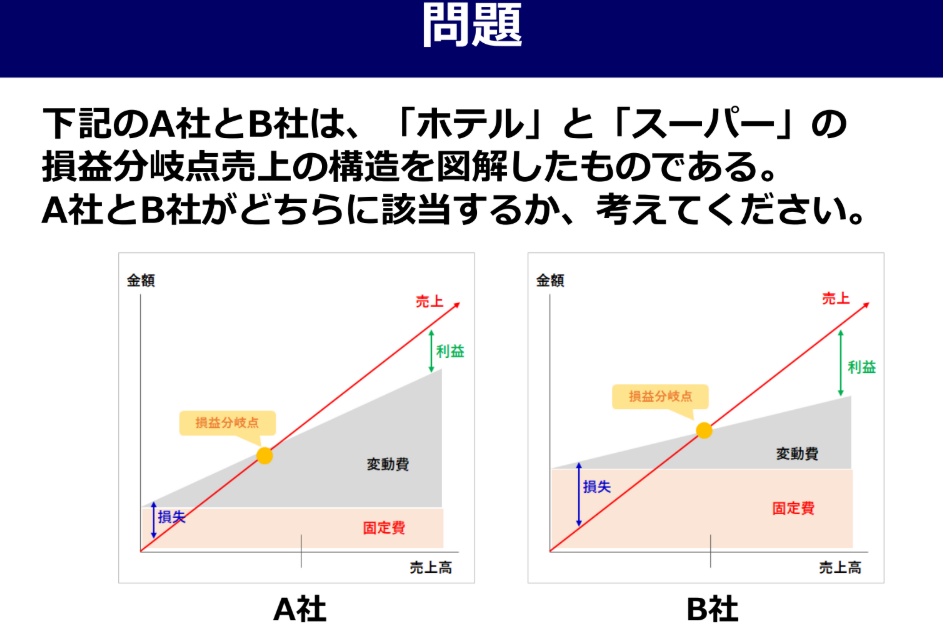
\includegraphics[width=12cm]{./images/mondai1.png}
  \caption{問題}
  \label{fig:break_even}
\end{figure}
\subsection{問題②}
タピオカミルクティーや
いっぱい400円

タピオカ1kg 1000円→いっぱい10円10g
ミルクティー1L 400円→いっぱい80円200ml
調味料一杯10円
紙コップ200Koiri 1000円→いっぱい5円
家賃月30万円 定休日無し，30日営業/月
社員給料計60万円/月
メンテナンス代5万円/月
水道光熱費10万円/月
一か月あたりの損益分岐点売上は?
変動費→105円\\
固定費→105万円\\
損益分岐点売り上げ数量 = 105万円 / (400 - 105) = 3560杯\\
損益分岐点売り上げ高 = 1050000 / (1 - 105/400) = 1,423,728円\\
一日当たりの損益分岐点売上数量= 3560 / 30 = 119杯\\
\section{DAY10}
人を動かす方法を学ぶ
\subsection{長野店の従業員改善}
アルバイト中心であり，正社員から指示を仰ぐことが多い．
ベテラン正社員は気性が荒い
→正社員を裏方の仕込みや商品補充を担当させ，フロアで問題が発生した場合に駆けつける形態に変更を行う．
そして，必要な日数店を閉めて，新人を教育をさせる．教育が終わったら一部のコーナーだけ開けて，店長が一人でトラブルがあってもカバーできる形態にする
\subsection{採用/教育/評価/報酬}
人事システム
\subsection{自分の体験から考察}
\subsubsection{実態}
採用→面接をして，会話をしている．紹介制度がある
教育→紙と動画のマニュアルがあり，新しいことをやるときには必ず定着するまで正社員がつく．
評価→定期的に行える業務内容をポイントで評価し，一定値を超えたら昇給するシステムがある．
報酬→時給制であり，昇給制度がある．

\subsection{リーダー}
先天的なものと後天的なものがある．
\subsubsection{先天的なもの}
決断力，やさしさ，意見を聞く etc...
\subsubsection{後天的なもの}
経験，知識，スキル etc...
\subsubsection{PM理論}
p→職務遂行
m→集団維持
pm→仕事に甘く，組織をまとめるのが下手
Pm→仕事はできるが，組織をまとめるのが下手
pM→仕事はできないが，組織をまとめるのが上手
PM→仕事もでき，組織もまとめるのが上手
リーダーに求められるのはその場に応じて変化する．
Pm型が重宝される場面も．
\section{DAY11}
フォロワーの重要性
\subsection{誘導方法}
ナッジ理論
\subsubsection{ナッジ理論とは}
人々の行動を強制するのではなく，選択肢の提示の仕方を工夫することで，望ましい行動を促す手法
命令よりも効果的\\
Nudge = ひじで軽くつつく\\
選択の自由を残したうえでよりよいものに気づかせる誘導．
\subsection{EASTフレームワーク}
Easy 簡単にする\\
Attractive 正しいインセンティブを\\
Social 正しい行動を示して\\
Timely タイムリーに
\subsubsection{Easy}
選択肢を減らす，デフォルトを設定する，行動を簡単にする
\subsubsection{Attractive}
報酬を与える，損失回避を利用する，感情に訴える
\subsubsection{Social}
社会的規範を利用する，行動を可視化する，協力を促す
\subsubsection{Timely}
適切なタイミングで情報を提供する，計画を促す，行動の直前に介入する
\section{DAY12}
集団意思決定\\
個人でやるよりも，集団でやったほうが良い意思決定ができる．
\section{DAY13(交渉)}
交渉を「対立や駆け引き」ではなく，「よりよい未来を創出する対話述」として捉え直し，その理論と実践スキルを身に着けること
\begin{itemize}
  \item 交渉の全体像を理解し，自分の立ち位置を客観的に把握するための重要概念(BATNA，ZOPA)を習得する．
  \item 「対立」を「協力」に変える思考法を学ぶ世界基準の交渉理論を学び，対立的な状況から，お互いにとって有益な解決策を見出すスキルを身に着ける．
  \item 交渉の場で使える具体的なテクニック(アンカリング，ミラーリング，ラベリングなど)を習得し，実践的な交渉力を高める．
\end{itemize}
今回の講義では，価値創造型交渉を中心に学ぶ．
\subsection{交渉の理論(フレームワーク)}
交渉の二つのタイプ:「奪い合い」か「価値創造」か
\begin{itemize}
  \item 価値分配型交渉(ディストリビューショナル・ネゴシエーション)
  \item 価値創造型交渉(インテグラティブ・ネゴシエーション)
\end{itemize}
\subsubsection{価値分配型交渉}
固定された大きさのパイを，いかに多く奪うかという「ゼロサムゲーム」\\
特徴:Win-Loseの関係になりやすい．自分の利益が相手の損失に直結する．
\subsubsection{価値創造型交渉}
協力してパイそのものを大きくし，分け前を増やす「プラスサムゲーム」
特徴:Win-Winの関係を目指す．複数の論点を組み合わせ，お互いの利益を最大化する．
\subsection{ケーススタディ(転職)}
BATNAとは?→Best Alternative to a Negotiated Agreement(最善の代替案)\\
交渉が決裂した場合にとることができる最善の代替案\\
例→アルバイトの面接．ほかにも応募できる\\
BATNAが多ければ多いほど交渉で有利に働く．\\
BATNAが弱いと，相手の無理な要求を受け入れざるを得なくなる．\\
RVAとは?→Reservation Value(最低ライン)\\
BATNAが最低ラインになる可能性があるが，ほかの視点からも考慮した際に，
最低ラインが変化する可能性がある．\\
例→転職の面接で，給料以外にも勤務地，福利厚生なども考慮すると，600万のA社よりもB社なら580万が最低ラインになる可能性もある．\\
悪い条件 << RV << BATNA << 理想条件\\
ここまでは自分の視点であったが，次は相手の視点で考える．
ZOPAとは?→Zone of Possible Agreement(合意可能領域)\\
相手のRVと自分のRVの間をZOPAという．\\
例)アルバイト面接\\
応募者の留保価値:時給800円 << ZOPA << 1200円:雇用者の留保価値\\
ZOPAの重要性\\
ZOPAが存在しない場合，交渉は決裂する．\\
ZOPAが存在する場合，交渉は合意に達する可能性がある．\\
\subsection{価値創造の方法①}
[1]パイを大きくする．
①複数の価値の論点を交渉のテーブルに載せる．
例(ZOPAが価格のみの焦点の場合，納期や品質という新たな価値をテーブルの交渉にあげる)
②価値の時間軸を変える．
短期的には譲れない価値も，長期的には譲れる可能性がある．
例)短期手には年収600万でいいが，○○を実現して，○○えんの利益をもたらしたら，年収800万にしてほしい．
[2]相手との違いに着目する
自分にとって重要で，相手にとって重要でないもの，相手にとって重要で，自分にとって重要でないものを
見つけ，妥協点を探る．
\subsection{交渉の準備}
交渉の成果の8割はテーブルに着く前の「準備」で決まると言われています．
\begin{itemize}
  \item 利害関係の分析
  \item BATNAの確認
  \item 留保価格の設定
  \item ZOPAの予測
\end{itemize}
利害関係を丁寧に分析することで，留保価格を複数設けることが出来る．(例:価格，品質，納期など)
\subsection{練習}
一月の試験期間直前(お店は繁忙期)
\section{DAY14(企業倫理)}
ある従業員のミスから，劇薬物の製造を担っている長野市の科学薬品工場にて爆発が起きた．
そして残念なことに，三人の従業員が死亡した．しかし会社は外部に対して全くコメントを出さなかった．
この場合，どんな感情を抱くだろうか．
どのような社会的な制裁が行われるのだろうか．
\subsection{広報からの倫理観}
\subsubsection{広報とは}
アカウンタビリティを発揮し，ステークホルダーとの信頼関係を構築/維持すること．\\
アカウンタビリティ→説明責任(自らの社会的責務の重大さを自覚して責務を推敲するとともに，
その責務から逸脱した場合には，自己の債務として逸脱を解消し，説明を行うこと．)\\
ステークホルダー→企業を取り巻く利害関係者のこと．\\
広報とは，企業倫理にかかわってくる重大な要素である．
\subsection{演習}
実際の広報業務をリアルに体験してみよう．
先ほどの化学薬品工場での爆発から一か月が経過．これまで一切工法をしてこなかったため，外部のステークホルダーから，猛烈な批判を受けている状況です．そこで急遽，記者会見を開くこととなりました．
\subsubsection{寸劇の内容}
企業側vs取材側の対決(x2回)を行う．10分間の制限時間の中で取材側は企業側を攻めていただき，企業側は取材側の攻撃を防御してもらいます．
最終的に，企業側に一定の理解を示すことが出来たか一般市民の方に判断してもらいます．
ただし途中で，取材側が勝利する条件\\
➀社長に「辞任します」と言わせた場合\\
➁会社側の誰かが、１００万円以上の\\
何らかの賠償を約束させた場合\\
コンプライアンスの重要性，守ることの難しさ
\end{document}